\documentclass[../all.tex]{subfiles}
\begin{document}
%%%%%%%%%%%%%%%%%%
    \section{Trolls Detector}
%%%%%%%%%%%%%%%%%%
	
	Troll Detector pretende ayudar a descubrir mentiras en Twitter o si más no, dar o quitar veracidad a las noticias que leemos en las redes sociales, concretamente en Twitter.\\
	
	Este proyecto consta de cuatro grandes fases donde se intentara conseguir el objetivo de si un tweet de una persona es falso o no. Estas cuatro fases se dividen en:
	
	\begin{enumerate}
		\item \textbf{Fase 0}, donde se tendrá que obtener  los últimos tweets de esa persona así como la creación y obtención de los diccionarios. Se llama fase 0 por ser una tarea previa  a todo el análisis y ser la parte mecánica o tarea sucia del trabajo donde no hay realmente un análisis de la información más allá de descartar todas aquellas palabras cuya aportación de información es nula (como seria el caso de artículos y preposiciones entre otras).
		
		\item La siguiente fase, \textbf{fase 1}, es la encargada de decir sobre que estamos hablando, en este trabajo acotado, nos dirá unicamente sobre que deporte o deportes habla esa persona en su Twitter usando la hipótesis propia inicial de que una persona no puede saber de todo o si más no, solo puede ser experto en un acotado número de deportes.
		
		\item A continuación, la \textbf{fase 2} pretende saber el tono/sentimiento con el que el autor del tweet lo esta escribiendo. Esto se hace con una hipótesis propia donde se especula que cuando estamos enfadados se escribe lo primero que pensamos e igual no se ciñe del todo a la realidad así como, cuando estamos alegres lo publicamos pensando que es verdad aunque puede que nosotros mismos estamos equivocados y escribamos una mentira. Esta fase se encuentra con muchos problemas como la ironía o la mala sintaxis y de más problemas que serán comentados más adelante.
		
		\item Para finalizar, la \textbf{fase 3}, donde se tendrá que recopilar la información anterior, contrastar si la cuenta que lo escribe es un perfil verificado o no, dado que las cuentas verificadas suelen ser de gente pública y por lo tanto, si cuentan mentiras, tendrán un castigo social más importante que si lo escribe alguien cuyo nombre no figura en Twitter. Se detectarán también aquellos usuarios que siempre estén al ataque contra otros o que escriban siempre de una forma furiosa (\textit{haters})y los perfiles que intenten hacer SPAM o decir siempre lo mismo. Por último se detectaran aquellos perfiles que sean usados para espiar o los llamados \textit{bots}.
		
	\end{enumerate}
	\newpage
	En la siguiente figura se puede observar un esquema general del proyecto para hacerse una idea de como funciona.
	
	\begin{figure}[H]
		\centering
		\includegraphics[height=14cm, width=11cm]{imgs/generalSchema.png}
		\caption{Esquema general del proyecto}
	\end{figure} 
	
\newpage
\subsection{Tecnologías utilizadas en todas las fases}
	En este apartado se darán a conocer las tecnologías usadas para la implementación del trabajo y su pertinente justificación. Se explican por separado las librerías de python y clases propias utilizadas en cada fase del proyecto.\\
	
	Python y R son los lenguajes de programación más usadso en \textit{data science}. Para este proyecto se ha escogido el uso de Python dado que\cite{RvsPython1}\cite{RvsPython2}:
	\begin{enumerate}[resume]
		\setcounter{enumi}{0}
		\item Python es fácil de utilizar:  Python tiene una reputación de ser fácil de aprender. Con una sintaxis legible, \item Python es ideal para principiantes o para científicos de datos que desean adquirir conocimiento en este lenguaje.
		\item Python es versátil: Como un lenguaje de propósito general, Python es una herramienta rápida y potente que tiene mucha capacidad. No importa cual sea el problema que quieras resolver, Python puede ayudarte a realizar la tarea, esto gracias a la gran cantidad de librerías con las que cuenta.
		\item Python es mejor para construir herramientas de análisis: R y Python son bastante buenos si desea analizar un conjunto de datos, pero cuando se trata de construir un servicio web para que otros utilicen los métodos desarrollados, Python es el camino a seguir.
		\item Visualización de datos con Python: En este aspecto es donde R generalmente le gana a Python. R tiene un amplio rango de herramientas de visualización, tales como, ggplot2, rCharts y googleVis. Más aunque \item Python no se presta en forma natural para la visualización, tiene una amplia gama de librerías disponibles, tales como Matplotlib, Plot.ly y Seaborn.
		\item La comunidad de Python esta creciendo: Python tiene una gran comunidad, que incluye una fuerte y creciente presencia en la comunidad de las ciencias de datos. PyPi es un lugar útil para explorar todo el alcance de lo que está desarrollando la comunidad.
		\item Python es mejor para Deep Learning: Hay muchos paquetes, como Theano, Keras y TensorFlow, que hacen que sea realmente fácil crear redes neuronales profundas con Python, y aunque algunos de estos paquetes están siendo portados a R, el soporte disponible en Python es muy superior.
	\end{enumerate}
	\newpage
    \subsubsection{MongoDB}
        MongoDB es un sistema de bases de datos NoSql de código abierto orientado a documentos. En lugar de almacenar la información en tablas como se haría en una base de datos relacional, MongoDB guarda la información en forma de documentos JSON, haciendo que la integración de este sistema de información sea mucho más simple y rápido que otros sistemas de bases de datos.\\
        
        MongoDB ha sido muy útil para almacenar de manera eficiente grandes conjuntos de tuits. Para trabajar con este sistema de bases de datos se ha empleado la librería PyMongo, que es la distribución para Python recomendada en la web oficial de MongoDB y que contiene todas las herramientas necesarias. Para el proyecto se ha empleado la versión 3.0.4 de MongoDB.\\
        
        MongoDB es un sistema fácil de utilizar y que funciona muy bien para guardar textos pero vamos a ver una tabla donde se puede comparar una base de datos como MongoDB con una SQL\cite{mongosql}.
        
        \begin{center}
            \begin{tabular}{ | m{3cm} | m{4cm}| m{4cm} | } 
                \hline
                \textbf{Feature} & \textbf{NoSQL Database} & \textbf{SQL Database} \\ 
                \hline
                Performance & High \checkmark & Low \\ 
                \hline
                Reliability & Poor & Good \checkmark \\ 
                \hline
                Availability & Good & Good \\ 
                \hline
                Consistency & Poor & Good \checkmark \\ 
                \hline
                Dara storage & Optimized for huge data \checkmark & Medium sized to large  \\ 
                \hline
                Scalability & High \checkmark & High but expensive  \\ 
                \hline
            \end{tabular}
        \end{center}
    \newpage
    \subsubsection{Pymongo 3.7.1}
        Pymongo es una librería de Python para poder conectarnos a una base de datos MongoDB.
        Para utilizar esta librería se utilizará una clase propia\cite{PyMongo}.
        \begin{figure}[H]
        	\centering
        	\includegraphics[height=13cm, width=15cm]{imgs/DB_class.png}
        	\caption{Clase DB utilizada para la comunicación entre el programa y la base de datos en MongoDB}
        \end{figure}
        
    \subsubsection{AVL Tree}
        
    	Todas las palabras están guardadas en una base de datos MongoDB pero con la finalidad de hacer la búsqueda más rápida una vez se consultan por primera vez se quedan guardadas en un árbol propio, concretamente en un AVL tree. \\
    	
    	Un árbol es un tipo abstracto de datos (TAD) muy utilizado que imita la estructura jerárquica de un árbol, con un valor en la raíz y subárboles con un nodo padre, representado como un conjunto de nodos enlazados.\\
   
    	La ventaja que tiene este tipo de árboles (AVL) es que están siempre equilibrados de tal modo que para todos los nodos, la altura de la rama izquierda no difiere en más de una unidad de la altura de la rama derecha o viceversa. Gracias a esta forma de equilibrio (o balanceo), la complejidad de una búsqueda en uno de estos árboles se mantiene siempre en orden de complejidad O(log n). El factor de equilibrio puede ser almacenado directamente en cada nodo o ser computado a partir de las alturas de los subárboles.\\
    	
    	\begin{figure}[H]
    		\centering
    		\includegraphics[height=10cm, width=13cm]{imgs/AVLtree_example.png}
    		\caption{Ejemplo AVL Tree}
    	\end{figure}
    	
    	Como se puede observar en la figura anterior, un árbol es unicamente una estructura de datos ordenada. En la figura es un orden numérico (de menos a más valor)  y el árbol utilizado en este trabajo está ordenado alfabéticamente. Con este árbol tendremos un coste inicial de creación pero luego el coste medio de la búsqueda de palabras será mucho menor.
    	\begin{figure}[H]
    		\centering
    		\includegraphics[height=13cm, width=11cm]{imgs/avl_class.png}
    		\caption{Diagrama de la clase propia AVL-TREE utilizada para la interacción con el árbol}
    	\end{figure}
    
\newpage
\subsection{Fase 0 - Extracción de la información y creación de los datasets}
    \subsubsection{Concepto}
        Esta primera fase 0 o fase inicial se irá modificando a lo largo de la implementación según se necesite. Pretende englobar tanto la extracción de los tweets como la creación de los diccionarios.\\
        
        Se pretende así que cada deporte tenga tres diccionarios asociados (palabras excluyentes, palabras vinculantes principales y palabras vinculantes secundarias). También se tendrán diccionarios para el análisis de las frases; palabras vacías, que son aquellas palabras que no aportan nada a la hora de clasificar el texto como podrían ser artículos y preposiciones.Por último se tendrá un diccionario asociado a cada uno de los sentimientos a analizar; alegría, amor, enfado, miedo, sorpresa y tristeza.\\
        
        Esta fase también es la encargada de la extracción de los tweets, no solo los X últimos del usuario para saber de que deportes habla sino también de guardar información sobre el usuario (como por ejemplo si el perfil se trata de una cuenta verificada), de si el tweet se trata de un retweet entrar en el perfil del usuario que lo ha publicado y hacer lo mismo que si fuese está persona inicial y por último comprobar los hashtags que ese tweet pueda contener.
		
    \newpage 
    \subsubsection{Software}
        El esquema de esta fase se puede ver en la siguiente imagen:\\
        \begin{figure}[H]
        \centering
            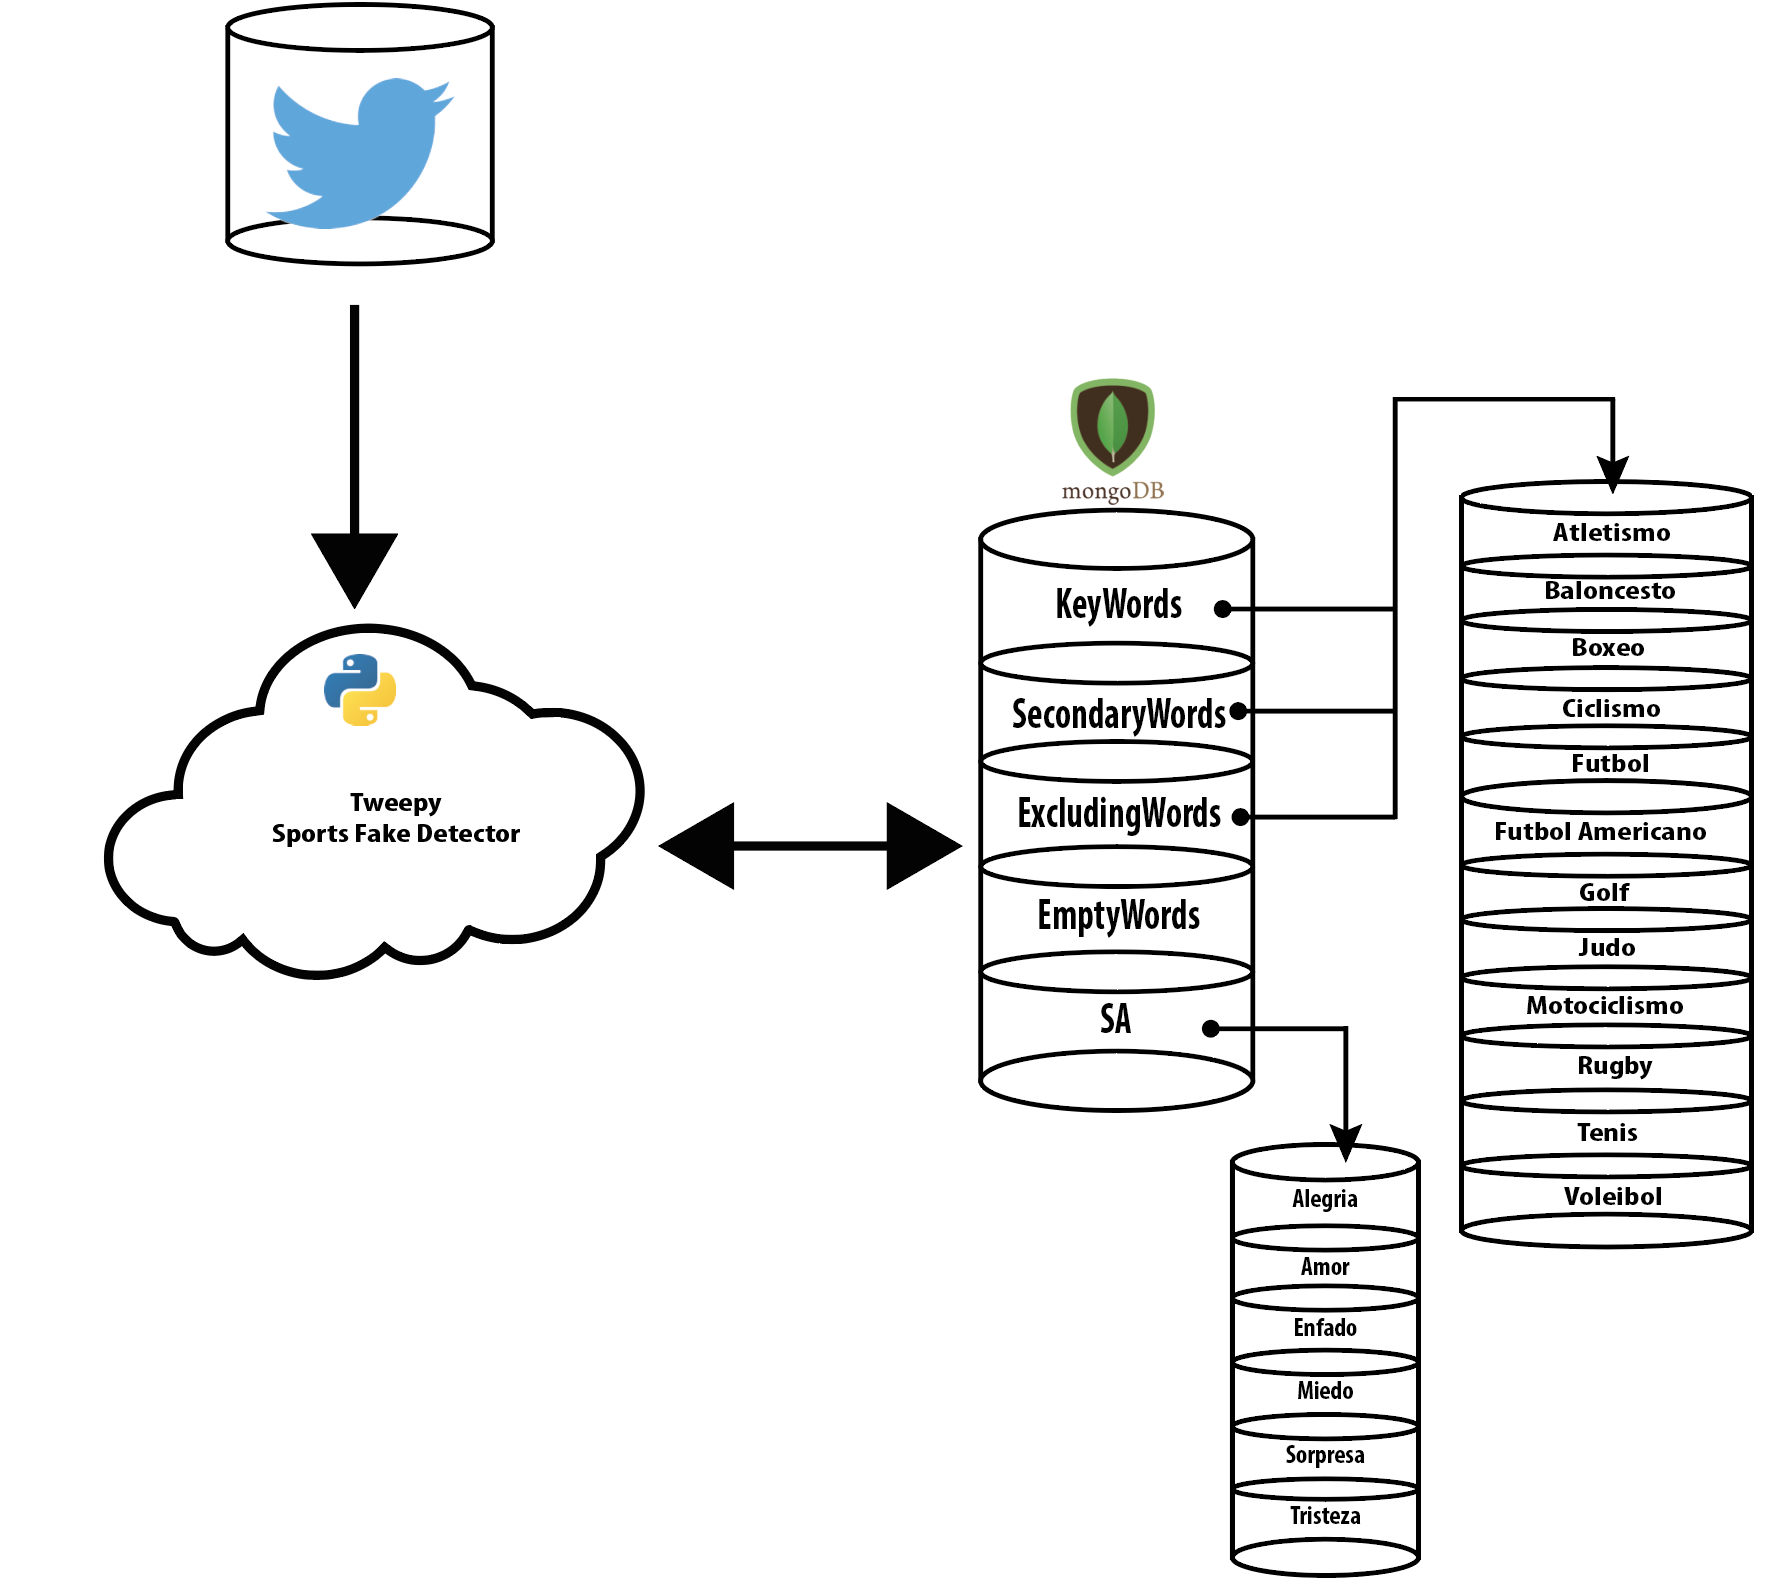
\includegraphics[height=13cm, width=15cm]{imgs/extraccionTwitter.png}
            \caption{Estructura de extracción de tweets y interacción con diccionario}
        \end{figure}
        Donde se puede ver que se extrae la información de twitter a través de la librería tweepy, se proceso con el detector de mentiras y se interacciona con la base de datos donde previamente se habían guardado los diccionarios.\\
        Las tablas de la base de datos son las siguientes:
        \begin{figure}[H]
        \centering
            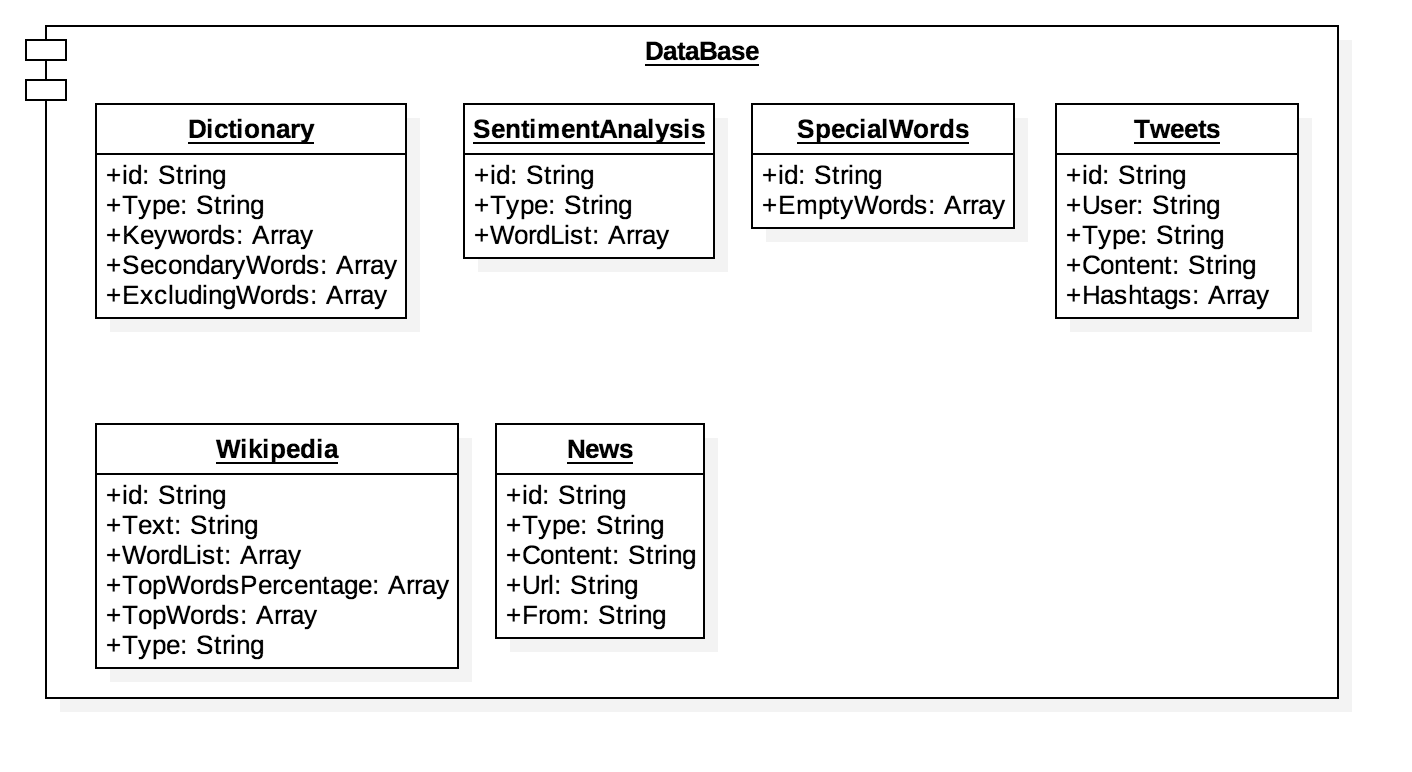
\includegraphics[height=15cm, width=15cm]{imgs/DB.png}
            \caption{Tablas en la base de datos del proyecto}
        \end{figure}
	    \paragraph{Wikipedia 1.4.0}
		    Está librería se empezó a usar con la finalidad de crear diccionarios automáticamente, simplemente coger todas las palabras que salen de una búsqueda en wikipedia, excluir todos los artículos, proposicionales y palabras que no aportan valor de clasificación.\\
		    
		    De todas las palabras obtenidas se cogían el 30\% de las palabras más repetidas. Esto permitió empezar a hacer pruebas de los algoritmos pero se descarto por falta de precisión y se empezó a hacer un diccionario propio que ganó riqueza por algunas palabras encontradas gracias a este algoritmo\cite{PyWiki}.
    	\newpage
       	\paragraph{Pymongo 2.7}
       		Pymongo es una librería de Python para poder conectarnos a una base de datos MongoDB. A continuación se muestra como hacer las principales operaciones con la librería\cite{PyMongo}.\\
       		\begin{figure}[H]
       			\centering
       			\includegraphics[height=10cm, width=9cm]{imgs/pymongoConnect.png}
       			\caption{Conectar con la Base de Datos}
       		\end{figure}
	       	\begin{figure}[H]
	       		\centering
	       		\includegraphics[height=8cm, width=8cm]{imgs/pymongoGet.png}
	       		\caption{Obtener el diccionario de nuestra BBDD}
	       	\end{figure}
	       \begin{figure}[H]
	       	\centering
	       	\includegraphics[height=13cm, width=13cm]{imgs/pymongoInsert.png}
	       	\caption{Insertar en la BBDD}
	       \end{figure}
       
       \newpage
       \paragraph{Tweepy 3.5}
            Tweepy es una librería de código abierto para Python que incluye todo el conjunto de funciones necesarias para comunicar con Twitter mediante las API's definidas por este. Las funciones definidas por Tweepy simplifican la conexión y búsquedas con Twitter. Por ejemplo, toda la conexión con Twitter debe estar certificada con un autor y, mientras que por defecto habría que configurar esta conexión mediante otra librería como sería Python-Auth y establecer cada conexión manualmente, Tweepy simplifica esto con unas funciones que simplemente esperan está autenticación como parámetro para poder configurarlo automáticamente. Estos parámetros son 4 tokens necesarios y en el caso de la búsqueda solo tenemos que indicarle los parámetros que solicita Twitter, toda la complejidad de las conexiones la trata internamente simplificando el trabajo inmensamente. Para el proyecto se ha empleado la versión 3.3 de Tweepy\cite{Tweepy}.
            \begin{figure}[H]
            	\centering
            	\includegraphics[height=7cm, width=7cm]{imgs/twitter_class.png}
            	\caption{Diagrama de la clase propia Twitter encargada de la comunicación con twitter mediante la librería tweepy}
            \end{figure}
        

\newpage    
\subsection{Fase 1 - Clasificación de texto según temática}
    \subsubsection{Concepto}
    	Para la clasificación de los tweets según su temática se hará uso de diferentes algoritmos y técnicas con la finalidad de conocer sobre qué temas escribe cada usuario de Twitter. La finalidad de esta fase por una parte es acotar los temas sobre los que habla cada usuario dada la suposición que lo más común en usuarios de Twitter (si nos centramos en los deportes) es que les guste mucho uno o dos deportes y sepan mucho de ellos y que luego sean simpatizantes de otros deportes. Por ejemplo en mi caso me gusta mucho el fútbol y el rugby y a veces miro el baloncesto o las carreras de motos gp pero no entiendo tanto de esos deportes como de mis favoritos. \\
    	
    	Para ello esta fase se centrará en recopilar los últimos tweets de un usuario, analizar sus \textit{hastags}, investigar la posible mención de usuarios en los tweets y averiguar también los deportes de aquel usuario y por último  si hizo algún \textit{retweet}  obtener la información sobre la otra cuenta obtenida en la fase anterior.\\
    	
    	Con el fin de conseguir todo esto se aplicarán diferentes técnicas para obtener lo que realmente nos interesa de cada tweet (palabras clave, \textit{hastags}, menciones a otros usuarios, etc) y una vez extraídas y \textit{tokenizadas} se aplicarán diferentes técnicas para su clasificación como sería primero eliminación de las palabras que no nos interesan, aplicación de diferentes algoritmos como Naive Bayes y el uso de un diccionario propio con palabras clave, palabras secundarias y palabras excluyentes de cada deporte.
    	
    \newpage
    \subsubsection{Software}
    	Para esta fase damos por sentado que ya tenemos acceso a la API de Twitter para obtener los tweets. Se ha decidido descargar los 20 tweets de cada usuario, teniendo en cuenta que si un tweet tiene un \textit{hashtag} o algún usuario se investigara también ese caso, se cree que ya será suficiente pero si los resultados (porcentaje del deporte al que pertenece) no es suficiente se cogerán 10 más.\\
    	
    	Por cada tweet se elimina las palabras que se cree que no aportan nada. Estas palabras se encuentran en la base de datos de MongoDB con el nombre de \textit{emptyWords} y para acceder a ellas se hace mediante la librería \textit{pymongo}. También se eliminan los signos de puntuación mediante la combinación de las librerías \textit{re} y \textit{string}. Por último se duplica la frase pero esta vez solo con la raiz de cada palabra, esto se conseguirá con la librería \textit{SnowballStemmer} la cual se puede utilizar en Español aunque no se obtienen los mejores resultados con ella.\\
    	
    	Una vez se tienen las palabras clave de cada frase se analiza con \textit{Naive Bayes}, SVM y con el diccionario propio creado.
    	
        \begin{figure}[H]
        	\centering
        	\includegraphics[height=13cm, width=13cm]{imgs/softwareFase1.png}
        	\caption{Diagrama fase 1 clasificación de texto según temática}
        \end{figure}
    
    	\newpage
        \paragraph{Stemmer}
        	Por razones gramaticales, los documentos van a utilizar diferentes formas de una palabra, como jugar, juegan y jugaron o jugador y jugadores. Además, hay familias de palabras derivadas relacionadas con significados similares, como vivir y convivir. En muchas situaciones, parece que sería útil buscar una de estas palabras para devolver documentos que contengan otra palabra en el conjunto.\\
        	
        	El objetivo tanto de la derivación (stemmer) como de la lematización (lemmatization) es reducir las formas flexivas y, a veces, las formas derivadas de una palabra a una forma básica común.\\
        	
        	Sin embargo, las dos palabras difieren en su forma de hacerlo. Stemming usualmente se refiere a un crudo proceso heurístico que elimina los extremos de las palabras con la esperanza de lograr este objetivo correctamente con un alto porcentaje, y a menudo incluye la eliminación de los afijos derivacionales. La lematización generalmente se refiere a hacer las cosas correctamente con el uso de un vocabulario y un análisis morfológico de las palabras, normalmente con el objetivo de eliminar solamente las terminaciones  y devolver la forma base o diccionario de una palabra, lo que se conoce como el lema (lemma).\\
        	
        	Como este trabajo esta en castellano, una lengua muy rica en su vocabulario y derivaciones, se ha optado por usar un Stemmer y no un lematizador dado que se obtienen mejores resultados.\\
        	
        	\begin{figure}[H]
        		\centering
        		\includegraphics[height=13cm, width=15cm]{imgs/stemExampleCode.png}
        		\caption{Código ejemplo utilización VADER}
        	\end{figure}
        	\begin{figure}[H]
        		\centering
        		\includegraphics[height=15cm, width=16cm]{imgs/stemExampleOutput.png}
        		\caption{Output ejemplo utilización VADER}
        	\end{figure}
        	
        	

        \paragraph{Naive Bayes}
        
        	El clasificador Naive Bayes es un clasificador probabilístico que se basa en el teorema de Bayes con suposiciones de independencia. Es una de las técnicas de clasificación de texto más básicas con varias aplicaciones en la detección de spam en el correo electrónico, clasificación de correo electrónico personal, categorización de documentos, detección de lenguaje y detección de sentimiento. \\
        	
        	Como se ha comentado se basa en el teorema de Bayes así que primero lo comentaremos y se usará como ejemplo la clasificación de texto. Se usa para predecir la probabilidad condicional de que un documento pertenezca a una clase P(c{\tiny i}$|$d{\tiny j}) a partir de la probabilidad de los documentos dada la clase P(d{\tiny j} $|$c{\tiny i}) y la probabilidad a priori de la clase en el conjunto de entrenamiento P(c{\tiny i})\cite{naiveBayes}.
        	
        	\begin{figure}[H]
        		\centering
        		\includegraphics[height=5cm, width=5cm]{imgs/naiveBayesEquation.png}
        		\caption{Formula Naive Bayes}
        	\end{figure}
        	
        	Dado que la probabilidad de cada documento P(d{\tiny j}) no aporta información
        	para la clasificación, el término suele omitirse. La probabilidad de un documento
        	dada la clase suele asumirse como la probabilidad conjunta de los términos que
        	aparecen en dichos documentos dada la clase y se calculan como:
        	\begin{figure}[H]
        		\centering
        		\includegraphics[height=5cm, width=5cm]{imgs/multinomialBayesEquation.png}
        		\caption{Formula Multinomial Bayes}
        	\end{figure}
        
        	Este algoritmo también se usará en la fase 2 para el análisis del sentimiento.
            
        \newpage
	    \paragraph{Support Vector Machine (SVM)}
	    
		    Las Máquinas de Vectores Soporte, creadas por Vladimir Vapnik, constituyen un método basado en aprendizaje para la resolución de problemas de clasificación y regresión. En ambos casos, esta resolución se basa en una primera fase de entrenamiento (donde se les informa con múltiples ejemplos ya resueltos, en forma de pares (problema, solución)) y una segunda fase de uso para la resolución de problemas. En ella, las SVM se convierten en una “caja negra” que proporciona una respuesta (salida) a un problema dado (entrada)\cite{svmexplicacion}.\\
		    
		    Dado un conjunto de puntos, subconjunto de un conjunto mayor (espacio), en el que cada uno de ellos pertenece a una de dos posibles categorías, un algoritmo basado en SVM construye un modelo capaz de predecir si un punto nuevo (cuya categoría desconocemos) pertenece a una categoría o a la otra.\\
		    
		    Como en la mayoría de los métodos de clasificación supervisada, los datos de entrada (los puntos) son vistos como un vector p-dimensional (una lista ordenada de p números). La SVM busca un hiperplano que separe de forma óptima a los puntos de una clase de la de otra, que eventualmente han podido ser previamente proyectados a un espacio de dimensionalidad superior. En la siguiente figura se puede observar ejemplos de como divide el espacio del conjunto de datos mas famoso del mundo en el ámbito de la inteligencia artificial (iris dataset) donde p sería tres. \\
		    
		    \begin{figure}[H]
		    	\centering
		    	\includegraphics[height=11cm, width=11cm]{imgs/SVMExplicacion.png}
		    	\caption{Ejemplo SVM\cite{svmexplicacion} con diferentes kernels.}
		    \end{figure}
		    
		    En ese concepto de "separación óptima" es donde reside la característica fundamental de las SVM: este tipo de algoritmos buscan el hiperplano que tenga la máxima distancia (margen) con los puntos que estén más cerca de él mismo. Por eso también a veces se les conoce a las SVM como clasificadores de margen máximo. De esta forma, los puntos del vector que son etiquetados con una categoría estarán a un lado del hiperplano y los casos que se encuentren en la otra categoría estarán al otro lado.
        
        \newpage
    	\paragraph{Random Forest Model}
    	
	    	Se trata de un método desarrollado por Leo Breiman y Adele Cutler en 2001 . Este método utiliza un conjunto (o bosque) de arboles de decisión para predecir un valor de salida. Para la clasificación de un nuevo ejemplo, cada árbol en el ensamble produce un voto, es decir, toma el ejemplo como entrada y produce una salida indicando a que clase pertenece. La decisión final del ensamble se realiza a partir de la clase con mayor cantidad de votos.\\
	    	
	    	La idea esencial del \textit{bagging} es promediar muchos modelos ruidosos pero aproximadamente imparciales, y por tanto reducir la variación. Los árboles son los candidatos ideales para el \textit{bagging}, dado que ellos pueden registrar estructuras de interacción compleja en los datos, y si crecen suficientemente profundo, tienen relativamente baja parcialidad. Producto de que los árboles son notoriamente ruidosos, ellos se benefician enormemente al promediar.\\
	    	
	    	Cada árbol es construido usando el siguiente algoritmo\cite{RandomForestModel}:
	    	\begin{enumerate}[resume]
	    		\setcounter{enumi}{0}
		    	\item Sea N el número de casos de prueba, M es el número de variables en el clasificador.
		    	\item Sea m el número de variables de entrada a ser usado para determinar la decisión en un nodo dado; m debe ser mucho menor que M
		    	\item Elegir un conjunto de entrenamiento para este árbol y usar el resto de los casos de prueba para estimar el error.
		    	\item Para cada nodo del árbol, elegir aleatoriamente m variables en las cuales basar la decisión. Calcular la mejor partición del conjunto de entrenamiento a partir de las m variables.
	        \end{enumerate}
        
        	Para la predicción un nuevo caso es empujado hacia abajo por el árbol. Luego se le asigna la etiqueta del nodo terminal donde termina. Este proceso es iterado por todos los árboles en el ensamblado, y la etiqueta que obtenga la mayor cantidad de incidencias es reportada como la predicción.
  		\newpage
    	\paragraph{XGBoost (Xtereme Gradient Boosting Model)}

			XGBoost significa eXtreme Gradient Boosting. Es el algoritmo que ha estado dominando recientemente los problemas Machine learning y las competiciones de Kaggle con datos estructurados o tabulares. XGBoost es una implementación de árboles de decisión con Gradient boosting diseñada para minimizar la velocidad de ejecución y maximizar el rendimiento. Posee una interface para varios lenguajes de programación, entre los que se incluyen Python, R, Julia y Scala.\\
			
			XGBoost es una implementación de código abierto popular y eficiente del algoritmo de árboles aumentados. La potenciación de gradientes es un algoritmo de aprendizaje supervisado que intenta predecir de forma apropiada una variable de destino mediante la combinación de estimaciones de un conjunto de modelos más simples y más débiles.\cite{XGBoost}.\\
			
		\begin{figure}[H]
			\centering
			\includegraphics[height=11cm, width=11cm]{imgs/xgboostAlgorithm.png}
			\caption{Ejemplo SVM\cite{XGBoost}}
		\end{figure}
			
			Internamente, XGBoost representa todos los problemas como un caso de modelado predictivo de regresión que sólo toma valores numéricos como entrada. Si nuestros datos están en un formato diferente, primero vamos a tener que transformarlos para poder hacer uso de todo el poder de esta librería. El hecho de trabajar sólo con datos numéricos es lo que hace que esta librería sea tan eficiente.
		 
		 \paragraph{Diccionario}
		
			Se ha creado un algoritmo propio muy sencillo y con el cual se han tenido muy buenos resultados. Recordemos que tenemos tres diccionarios por cada uno de los deportes (para la parte de clasificación de texto según la temática), uno con las palabras clave donde si se encuentra esa palabra ya sabremos con bastante seguridad que se trata de ese deporte, uno con palabras secundarias con el cual el que más repeticiones de palabras tenga será el deporte del cual se estará hablando y un diccionario de palabras excluyentes para poder romper posibles empates en cuanto palabras secundarias.
		


\newpage
\subsection{Fase 2 - Análisis del sentimiento}
    \subsubsection{Concepto}
    	En esta segunda fase se quiere analizar el comportamiento del usuario para analizar si es muy critico o si solo tiene buenas palabras para su equipo como seria el ejemplo de un aficionado extremista del Sevilla CF o el Real Betis Balompié donde su rivalidad es histórica y los cuales siempre tienen buenas palabras para su equipo y malas formas e incluso insultos hacía la otra afición.\\
    	
    	Para la realización de esta fase y poder analizar el sentimiento de los últimos tweets del usuario se hará uso de diferentes librerías como  \textit{VaderSetniment},  \textit{TextBlob} y  \textit{NLTK} para definir si su sentimiento es positivo, negativo o neutral y para dar un resultado más detallado y poder determinar si el sentimiento es de alegría, miedo, sorpresa y amor entre otros se utilizará un diccionario propio con palabras que definen cada uno de los sentimientos.\\
    	
    	 El primer estudio se hace para dar un resultado más preciso ya que si sale un sentimiento negativo pero una segunda clasificación de alegría sabremos que algo está mal y por otro lado si da que el sentimiento es negativo se buscará antes sentimientos como enfado o tristeza a los de amor y alegría.
    	 
    \newpage
    \subsubsection{Software}
    
    	Para esta frase se utiliza la frase entera sin modificar dado que las librerías \textit{VADER Sentiment} y \textit{Textblob} ya las tratan internamente. Con esto ya sabremos si la frase es positiva, negativa o neutral\cite{VADER}.\\
    	
    	Una vez sabemos si es positiva, negativa o neutral se utilizará la frase modificada por nosotros (sin las palabras que nosotros mismos hemos llamado palabras vacías) y se aplicará un algoritmo con el diccionario propio para saber si los tweets del usuario hablan de alegría, amor, enfado, miedo, sorpresa o tristeza.
        
        \begin{figure}[H]
        	\centering
        	\includegraphics[height=15.5cm, width=17cm]{imgs/softwareFase2.png}
        	\caption{Diagrama fase 2 análisis del sentimiento}
        \end{figure}
    
    	\newpage
        \paragraph{VADER Sentiment 3.3}
        
        	VADER (Valence Aware Dictionary and sEntiment Reasoner) es un léxico y una biblioteca de análisis de sentimiento basada en reglas. Sirve como herramienta de análisis de sentimientos basada en reglas que está específicamente adaptada a los sentimientos expresados en las redes sociales.\\
        	
        	 Es completamente de código abierto bajo la [Licencia MIT]. VADER puede incluir el sentimiento de los emoticonos (por ejemplo, :-)), los acrónimos relacionados con el sentimiento (por ejemplo, LOL) y la jerga (por ejemplo, meh).\\
        	 
        	 El método vaderSentiment() devuelve los valores para representar la cantidad de sentimiento negativo, positivo y neutral y también calcula el valor de sentimiento compuesto como un valor con signo para indicar la polaridad del sentimiento general.\\
        	 
        	 A continuación se muestra un ejemplo de utilización de VADER:
        	 \begin{figure}[H]
        	 	\centering
        	 	\includegraphics[height=15cm, width=16cm]{imgs/vaderExampleCode.png}
        	 	\caption{Código ejemplo utilización VADER}
        	 \end{figure}
        	\begin{figure}[H]
        		\centering
        		\includegraphics[height=15cm, width=16cm]{imgs/vaderExampleOutput.png}
        		\caption{Output ejemplo utilización VADER}
        	\end{figure}
        
		\newpage
        \paragraph{TextBlob 0.15.1}
        	TextBlob es una librería de Python (2 y 3) para procesar datos textuales. Proporciona una API simple para adentrarse en tareas comunes de procesamiento del lenguaje natural (NLP), como etiquetado parcial, extracción de frase nominal, análisis de sentimiento, clasificación y traducción\cite{TextBlob}.\\
        	
        	En esta fase se ha utilizado esta librería para traducir tweets de otros idiomas y para la clasificación del sentimiento se escogió esta librería porque que ofrece una API simple para acceder a sus métodos y realizar tareas NLP básicas.
        	
        \paragraph{NLTK 3.2.2}
			NLTK (Natural Language Toolkit) es una plataforma líder para construir programas de Python para trabajar con datos de texto natural. Proporciona interfaces fáciles de usar a más de 50 recursos léxicos como WordNet, junto con un conjunto de librerías de procesamiento de texto para clasificación, tokenización, derivación, etiquetado, análisis y razonamiento semántico, envoltorios para bibliotecas de PNL de fuerza industrial, y un foro de discusión activo\cite{NLTK}.\\
			
			Contiene una completa documentación (API). Está disponible para Windows, Mac OS X y Linux. NLTK es un proyecto gratuito y de código abierto que ha sido llamado ``una herramienta maravillosa para enseñar y trabajar en lingüística computacional usando Python'' y ``una biblioteca increíble para jugar con el lenguaje natural''.

        \paragraph{Diccionario}
        
            Para la implementación de este algoritmo, a diferencia de la fase anterior, solo tenemos un diccionario propio por cada una de las palabras. El algoritmo se basa simplemente en averiguar si las palabras escritas en el tweet se encuentran o no en alguno de los diccionarios implementados para cada uno de los sentimientos. Gracias al algoritmo VADER sentiment ya podemos hacer un primer descarte de sentimientos.
\newpage
\subsection{Fase 3 - Resultado del análisis}

		Esta última fase es donde se encuentra el cerebro de la aplicación, tendrá que recopilar la información anterior y decidir si la persona ha mentido o no. Se trata de la fase más complicada y que por ello conlleva más problemas. Si en las fases anteriores se tenía dudas se puede imaginar que si sumas un grado fiabilidad alto pero lejano al 100\% como nos ocurre con la clasificación de texto según la temática con una fiabilidad cercana al 50\% como tenemos en el análisis del sentimiento, lo que se obtiene es una fiabilidad aun menor y si a ello le sumas hipótesis propias que no tienen un grado de fiabilidad definido, lo que se acaba obteniendo es un \textit{cocktail} que habrá que saber manejar con cuidado.\\
		
		Las hipótesis mas relevantes a tener en cuenta son:
		\begin{enumerate}
			\item Una persona que opina de todo es más propensa a mentir aunque sea por desconocimiento de las cosas a una persona que opina sobre uno o dos deportes donde igual es periodista, jugador de ese deporte o un aficionado interesado profundamente a ese deporte.
			\item Un fanático o persona que habla sobre ese deporte y esta enfadado insulta y habla mal de los jugadores sin apenas pensar y no tiene por que ser verdad al igual que cuando escribe con miedo espera que ese texto escrito por él mismo no sea verdad.
			\item  Contrastar si el perfil que lo escribe es una cuenta verificada o no, dado que las cuentas verificadas suelen ser de gente pública y por lo tanto, si cuentan mentiras, tendrán un castigo social más importante que si lo escribe alguien cuyo nombre no figura en Twitter. 
			\item Si la persona que lo escribe es alguien importante del deporte suele tener muchos \textit{retweets} y por lo tanto numerosos tweets parecidos al suyo por lo tanto, si se busca ese \textit{hashtag} se deberían tener comentarios similares.
			\newpage
			\item Los textos con los emoticonos;
			\begin{figure}[H]
				\centering
				\includegraphics[height=4cm, width=6cm]{imgs/emotis.png}
			\end{figure}
			entre otros, suelen ser los escritos con hironía y por lo tanto, los más difíciles de clasificar.
			\item Si escribes mal de un equipo o jugador o deportista no pertenece a tu equipo o en el caso de las olimpiadas a tu país, no habría que hacer mucho caso de lo escrito dado que se escribirá en parte desde el rencor y so por lo contrario escribes bien sobre el habría que intentar detectar la hironía porque a no ser que haya hecho realmente el mejor partido o carrera de su vida, seguramente se habrá escrito una mentira.
		\end{enumerate}
	
	Finalmente este proyecto  pretende encontrar tres tipos de trolls:
	\begin{enumerate}
		\item Los mentirosos: Aquellos usuarios que digan mentiras en Twitter.
		\item Los furiosos:. Aquellos perfiles que siempre estén poniendo tweets de una forma furiosa o hiriente.
		\item Los \textit{spammers}: Aquellos tuiteros que continuamente dicen lo mismo.
	\end{enumerate}

		 

\end{document}
